\documentclass[10pt,a4paper]{article}
\usepackage[utf8]{inputenc}
\usepackage{amsmath}
\usepackage{amsfonts}
\usepackage{amssymb}
\usepackage{mathtools}
\usepackage{bm}
\newcommand\bigzero{\makebox(0,0){\text{\large 0}}}
\usepackage{graphicx}
\usepackage{epstopdf} 
\usepackage[justification=centering]{subfig}
\usepackage[T1]{fontenc}
\usepackage{lmodern}
\usepackage[backend=bibtex8,style=authoryear,hyperref=true,url=false,isbn=true,backref=true,maxcitenames=3,maxbibnames=100,firstinits=true,block=ragged]{biblatex}
%\usepackage[pdftex,ocgcolorlinks,colorlinks,linkcolor=DarkBlue,urlcolor=DarkGreen,citecolor=Black,linktoc=page,breaklinks]{hyperref}

\addbibresource{library.bib}


\newcommand{\vectornorm}[1]{\left\|#1\right\|}

\newcommand{\threepartdef}[6]
{
	\left\{
		\begin{array}{lll}
			#1 & \mbox{for } #2 \\
			#3 & \mbox{for } #4 \\
			#5 & \mbox{for } #6
		\end{array}
	\right.
}

\begin{document}
\title{Semester project}
\author{Espen Johansen Velsvik}
\maketitle

\section{Introduction}
\chapter{Introduction}
When an observer of an object moves relative to the object, there is an apparent relative motion in the image plane of the observer. The problem of determining this relative motion from a sequence of images is called the Optical Flow problem. The analysis is not so much dependent on prior knowledge of the scene, but on the image sequence itself. This independency makes it applicable in many different fields. More concisely, one wants to find flow vector components $u,v \in \mathbb{R}$ by looking at the change in brightness $f(x,t)$ at a specific pixel from one frame to another for $x \in \Omega$, where $\Omega$ is considered to be a rectangular domain. This is problematic because we can not independently determine a vector of 2 components using one constraint coming from the change in image brightness at a point $x \in \Omega$. Thus we need to impose other constraints to make the problem solvable.

Is there always a relationship between the change in the brightness and the movement of objects in the image? It is not hard to see that the answer is no. For instance, imagine rotating a uniform sphere exhibiting a nonuniform brightness pattern over its surface. This rotation is not observable in the image plane, and would result in zero optical flow. Also, if the illumination of the image scene changes rapidly, brightness changes in the image plane may not be due to moving objects. These examples illustrate that optical flow does not always correspond to the relative movement of an object. Nonetheless, in the following model for optical flow the image scene is assumed to be simple so that brightness changes can be directly related to object motion.    

\section{The Brightness constancy assumption}
\chapter{The Brightness Constancy Assumption}
\sectionmark{The Brightness Constancy Assumption}
The starting point for the variational approach to optical flow is the so called brightness constancy assumption of Horn and Schunck \cite{HS}. Let $f(x,t)$ be the grayscale value of some image sequence. To constrain the problem one makes an assumption regarding invariance in the brightness: a point moving with velocity $\frac{dx}{dt} = u(x,t)$ along the trajectory $x(t)$ over time $t$ does not change its appearance. This assumption is called the brightness constancy assumption, and it means that if the scene has the same lighting, then movement of an object along a trajectory does not change its brightness.
\section{The Data Term}
In mathematical notation this is (under perfect conditions) equivalent to the following:
\begin{align*}
\frac{d}{dt}f(x(t),t) = 0.
\end{align*}
By using the chain rule for differentiation, and defining $\frac{dx}{dt} = u$ and $\frac{dy}{dt} = v$, one gets
\begin{align*}
\frac{\partial f}{\partial x} u + \frac{\partial f}{\partial y} v + \frac{\partial f}{\partial t} = 0,
\end{align*}
or equivalently, by defining $\textbf{w} = (u,v)^T$, $\nabla f^T  \textbf{w} + f_t = 0$. Following the notation and terminology of Zimmer et al. \cite{zimmer2011optic}, the constraint coming from the brightness constancy assumption is called the data term $M(u,v)$.

\section{Penalizing the Data Term}
To minimize the data term above, Horn and Schunck used a quadratic penalizer, which is equivalent to least-squares minimization. Least-squares minimization is very sensitive to outliers. In the case of the data term, these outliers would be noise in the image (a pixel that jumps from low intensity to high intensity without corresponding to the motion of an object). Due to the poor robustness to outliers of least-squares minimization other penalization functions have been suggested. Black and Anandan \cite{Black199675} proposed several subquadratic penalizer functions, arguing that a subquadratic penalizer would improve the robustness in the presence of outliers. Letting
\begin{align*}
\rho(\textbf{w}) = \nabla f \cdot \textbf{w} + f_t
\end{align*}
and assuming the data term has some quadratic dependence on $\rho$, one can define
\begin{align}
\label{DataPenalize}
M(u,v) = \Psi_M(\rho^2),
\end{align}
where $\Psi_M$ is some penalizing function aiming to minimize $\rho$. Since the flow consists of 2 components, the brightness constancy assumption alone is not enough to determine the flow, but only the components of the flow in the direction of the gradient, or what is known as the normal flow. This is called the Aperture problem, and to be able to compute the components of the flow vector one needs another constraint. This other constraint is known as the smoothness constraint.

\section{The Smoothness constraint}
\chapter{The Smoothness Constraint}
\sectionmark{The Smoothness Constraint}
As noted in the previous section, the system does not admit a unique solution with the constraints given by the data term. A common approach, an idea introduced by Horn and Schunck \cite{HS}, is to incorporate a smoothness constraint in the model. This smoothness constraint, also called the spatial coherence assumption \cite{Black199675}, says that points can not move independently in the brightness pattern. There has to be some smoothness in the flow vector for points belonging to the same object. In other words, points on the same object moves with the same velocity. A natural way of obtaining a smoother solution would be to minimize some term depending on the sizes of the gradients $\nabla u$ and $\nabla v$. As noted by Horn and Schunck, this leads to problems where one would expect discontinuous flow patterns. This is the case in images where occlusions are present, for instance an image of an object moving in a snow storm. The smoothness terms considered here will be quadratic with respect to the gradient in each direction, thus it is convenient to write the smoothness term in the form
\begin{align}
\label{SmoothnessTerm}
V(\nabla u, \nabla v) = \nabla u ^T \Theta_u \nabla u + \nabla v ^T \Theta_v \nabla v.
\end{align}
The interpretation of the matrices $\Theta_u$ and $\Theta_v$ will become clear in the following section. 

\section{The variational formulation}
\chapter{Variational Formulation}
\sectionmark{Variational Formulation}
To combine the two constraints into one term we form a global energy function consisting of the data term and the smoothness term:
\begin{align}
E(u,v) = \frac{1}{2} \int_\Omega (M(u,v) + \frac{1}{\sigma^2} V(\nabla u, \nabla v)) \, dx \, dy,
\end{align}
where $\sigma > 0$ is a regularization parameter. The problem is now to find the minimum of the energy functional $E(u,v)$. From calculus of variations we have that if $\textbf{w}$ minimizes a functional
\begin{align*}
J(\textbf{w}) = \iint \limits_\Omega F(x,y,\textbf{w},\textbf{w}_x,\textbf{w}_y) \, dx \, dy,
\end{align*} 
then the first variation must be zero,
\begin{align*}
\delta J(\textbf{w}) = \frac{d}{d \epsilon} \left[ J(\textbf{w} + \epsilon \bm{\eta}) \right] = 0,
\end{align*}
for any arbitrary function $\bm{\eta}(x,y)$. We get
\begin{align*}
\delta J(\textbf{w}) =&  \iint \limits_{\Omega} \frac{d}{d \epsilon} F(x,y,\textbf{w} + \epsilon \bm{\eta}, \textbf{w}_x + \epsilon \bm{\eta}_x, \textbf{w}_y + \epsilon \bm{\eta}_y) \, dx \, dy \\
=&  \iint \limits_{\Omega} \bm{\eta} F_\textbf{w} + \bm{\eta}_x F_{\textbf{w}_x} + \bm{\eta}_y F_{\textbf{w}_y} \, dx \, dy \\
=& \iint \limits_{\Omega} \bm{\eta} F_\textbf{w} + \frac{d}{d x} (\bm{\eta} F_{\textbf{w}_x}) + \frac{d }{d y} (\bm{\eta} F_{\textbf{w}_y}) - \bm{\eta} \left( \frac{d}{d x} F_{\textbf{w}_x} + \frac{d }{d y} F_{\textbf{w}_y} \right) \, dx \, dy
\end{align*}
Now let $\Gamma_{E}$, $\Gamma_{W}$, $\Gamma_{N}$ and $\Gamma_{S}$ be the east, west, north and south boundary of our domain respectively. Then using Gauss' Theorem gives
\begin{align*}
& \iint \limits_{\Omega}  \frac{d}{d x} (\bm{\eta} F_{\textbf{w}_x}) + \frac{d }{d y} (\bm{\eta} F_{\textbf{w}_y}) \, dx \, dy \\ 
=  &\int_{\Gamma_{e}} \bm{\eta} F_{\textbf{w}_x} \, dx - \int_{\Gamma_{w}} \bm{\eta} F_{\textbf{w}_x} \, dx + \int_{\Gamma_{n}} \bm{\eta} F_{\textbf{w}_y} \, dy - \int_{\Gamma_{s}} \bm{\eta} F_{\textbf{w}_y} \, dy
\end{align*}
Using this result, we get
\begin{align*}
&\delta J(\textbf{w}) = \iint \limits_{\Omega} \bm{\eta} \left( F_\textbf{w} -  \frac{d}{d x} F_{\textbf{w}_x} - \frac{d }{d y} F_{\textbf{w}_y} \right) \, dx \, dy  \\ 
+ & \left( \int_{\Gamma_{E}} \bm{\eta} F_{\textbf{w}_x} \, dx - \int_{\Gamma_{W}} \bm{\eta} F_{\textbf{w}_x} \, dx + \int_{\Gamma_{N}} \bm{\eta} F_{\textbf{w}_y} \, dy - \int_{\Gamma_{S}} \bm{\eta} F_{\textbf{w}_y} \, dy \right) = 0.
\end{align*}
Since this must hold for any arbitrary function $\bm{\eta}(x,y)$ it follows that
\begin{align*}
F_{\textbf{w}} - \frac{d}{dx} F_{\textbf{w}_x} - \frac{d }{d y} F_{\textbf{w}_y} &= 0 \quad \text{in} \ \Omega \\
F_{\textbf{w}_x} &= 0 \quad \text{on} \ \Gamma_e \ \text{and} \ \Gamma_w \\
F_{\textbf{w}_y}& = 0 \quad \text{on} \ \Gamma_n \ \text{and} \ \Gamma_s
\end{align*}
This is called the Euler-Lagrange equation of variational calculus. From this result it is easy to see that the following must hold for our functional:
\begin{equation}
\label{EL}
  \begin{aligned}
\partial_{\textbf{w}} M - \frac{1}{\sigma^2}\left( \frac{d}{d x} \partial_{\textbf{w}_x} V + \frac{d}{d y} \partial_{\textbf{w}_y} V \right) &= 0 \quad \text{in} \ \Omega  \\
\partial_{\textbf{w}_x} V &= 0 \quad \text{on} \ \Gamma_E \ \text{and} \ \Gamma_W \\
\partial_{\textbf{w}_y} V &= 0 \quad \text{on} \ \Gamma_N \ \text{and} \ \Gamma_S
  \end{aligned}
\end{equation}
As previously noted, we are dealing with quadratic smoothness terms. Using the notation of (\ref{SmoothnessTerm}), the first equation in the Euler-Lagrange system can be written as
\begin{equation}
\label{EL_regu}
  \begin{aligned}
\partial_q M - \frac{1}{\sigma^2} \text{div} \left(\Theta_q \nabla q \right) = 0 \\
	\end{aligned}
\end{equation}
for $q \in u, v$. The matrix $\Theta_q$ is a diffusion matrix steering the direction of diffusion for each flow component. Its eigenvectors and corresponding eigenvalues gives the direction and magnitude of smoothing respectively. The theoretical framework presented up to this point is the same for all the methods considered here. The main distinction for each method will be across which boundaries the flow field is smoothed, that is, the choice of diffusion matrix. We start with the simplest choice; the uniform smoothness approach by Horn and Schunck.


\section{The approach by Horn and Schunck}
\chapter{The Approach of Horn and Schunck}
\chaptermark{The Approach of Horn and Schunck}
The research of Horn and Shunck has formed the basis of further research in the field of optical flow. They proposed the following quadratic penalized data term
\begin{align}
M(\textbf{w}) = (\nabla f^T \textbf{w} + f_t)^2,
\end{align}
which is equivalent to choosing
\begin{align*}
\Psi_M(\rho^2) = \rho^2
\end{align*}
in the framework of (\ref{DataPenalize}). The contribution to (\ref{EL}) from the model term is thus 
\begin{equation}
\begin{aligned}
\partial_{\textbf{w}} M = 2\nabla f(\nabla f ^T  \textbf{w} + f_t)
\end{aligned}
\end{equation}
The smoothness term used by Horn and Schunck is
\begin{align*}
V(\nabla u, \nabla v) = |\nabla u|^2 + |\nabla v|^2.
\end{align*}
This is a homogeneous regularizer which means that it applies an equal amount of diffusion in all directions. In the framework of (\ref{EL_regu}), this is equivalent to the diffusion matrices $\Theta_u$ and $\Theta_v$ being the identity matrix. Using this function as a flow regularizer gives
\begin{align*}
\partial_ {\textbf{w}_{x_i}} V = 2\textbf{w}_{x_i},
\end{align*}
for $x_i = x, y$. Dividing by 2 in all terms results in (\ref{EL}) taking the form 
\begin{equation}
\label{EL_HS}
\begin{aligned}
(f_x u + f_y v + f_t) f_x - \frac{1}{\sigma^2}(\frac{d}{d x} u_x + \frac{d}{d y} u_y ) &= 0  \quad \text{in} \ \Omega,  \\
(f_x u + f_y v + f_t) f_y - \frac{1}{\sigma^2}(\frac{d}{d x} v_x + \frac{d}{d y} v_y ) &= 0  \quad \text{in} \ \Omega  \\
\textbf{w}_{x} &= 0 \quad \text{on} \ \Gamma_e \ \text{and} \ \Gamma_w, \\
\textbf{w}_{y} &= 0 \quad \text{on} \ \Gamma_n \ \text{and} \ \Gamma_s,
\end{aligned}
\end{equation}
which can be seen as a system of coupled Poisson equations with Neumann boundary conditions:
\begin{align*}
-\frac{1}{\sigma^2} \Delta u + f_x ^2 u = - (F(v) + f_tf_x) \\
-\frac{1}{\sigma^2} \Delta v + f_y ^2 v = - (F(u) + f_tf_y) ,
\end{align*}
where $F(q) = f_xf_y q$.


\section{Discretizing the Horn and Schunck method}
\label{sec: disc}
Let now our image be of size m-by-n, and let $f^1$ and $f^2$ be the image at $t=1$ an $t=2$ respectively. Also, we flatten the regular 2-dimensional grid in $\Omega$ and consider now $(\xi^i)_ {i \in [mn]}$ so that $(\xi^i) = (x,y) = (\left \lfloor{i/m}\right \rfloor, i - \left \lfloor{i/m}\right \rfloor)$, when assuming the distance between vertical and horizontal grid points in $\Omega$ are 1. The corresponding vector representation of the image $f$ is denoted as $\textbf{f}(\xi^i) \in \mathbb{R}^{mn}$. Continuing this notation, the discrete flow values $\textbf{w}(\xi^i)$ is represented as the following vector in $\mathbb{R}^{2mn}$:
\begin{align*}
     \textbf{w}(\xi^i)=\begin{bmatrix}
         u(\xi^i)_{i\in [mn]}  \\
         v(\xi^i)_{i \in [mn]} \\
        \end{bmatrix}.
\end{align*}
For the discretization of the image gradients in (\ref{EL_HS}), the forward difference was used on $f^1$, producing the two vectors $\textbf{d}_x(\xi^i)$ and $\textbf{d}_y(\xi^i)$ in $\mathbb{R}^{mn)}$, where the gradients on the boundary are assumed to be zero. The time derivative $f_t$ is discretized using forward difference with time step $\Delta t = t_2 - t_1 = 1$ as shown below:
\begin{align*}
\textbf{c}(\xi^i) = \textbf{f}^2(\xi^i) - \textbf{f}^1(\xi^i),
\end{align*} 
where $\textbf{c}(\xi^i)$ is a vector in $\mathbb{R}^{mn}$. Normally when choosing derivative approximations one wants as high order as possible so that the truncation error goes to zero as one increases the number of grid points. In this case the number of grid points is fixed, so there is little to gain from choosing higher order approximations; it is best to choose the derivative approximation that results in the simplest discretization. Thus for the flow vector in (\ref{EL_HS}), the first derivative was approximated using backward difference, and the second was approximated using forward difference. Let now $L_x$ and $L_y$ be the matrices performing a forward difference on the components of the vector $\textbf{w}$ in $x$- and $y$-direction respectively. The gradient is then represented as
\begin{align*}
L \textbf{w}(\xi^i) = \begin{bmatrix}
         \tilde{u}_x(\xi^i)_{i\in [mn]}  \\
         \tilde{u}_y(\xi^i)_{i\in [mn]}  \\
         \tilde{v}_x(\xi^i)_{i\in [mn]} \\
         \tilde{v}_y (\xi^i)_{i\in [mn]} \\
        \end{bmatrix}
\end{align*}
where $\tilde{u}_x, \tilde{v}_x, \tilde{u}_y, \tilde{v}_y \in \mathbb{R}^{mn}$ are vector approximations to the derivatives. This means that $L$ is the following  block matrix:
\begin{align*}
L = \left[
\begin{array}{c c}
L_x & 0 \\
L_y & 0\\
0 & L_x \\
0 & L_y \\
\end{array}
\right].
\end{align*}

%\begin{align*}
%     \textbf{w}_x(\xi^i)=\begin{bmatrix}
%         u_x (\xi^i) \\
%         v_x (\xi^i)\\
%        \end{bmatrix} &\approx L_x \textbf{w}(\xi^i) = \begin{bmatrix}
%         \tilde{u}_x(\xi^i)  \\
%         \tilde{v}_x (\xi^i)\\
%        \end{bmatrix}  \\
%             \textbf{w}_y(\xi^i)=\begin{bmatrix}
%         u_y (\xi^i) \\
%         v_y (\xi^i)\\
%        \end{bmatrix} &\approx L_y \textbf{w}(\xi^i) = \begin{bmatrix}
%         \tilde{u}_y (\xi^i) \\
%         \tilde{v}_y(\xi^i) \\
%        \end{bmatrix},
%\end{align*} 
Since (\ref{EL_HS}) gives one set of equations for the interior nodes and one for the boundary nodes, these have to separated into two coupled systems. The interior system can be written as
\begin{align}
(D^T D + \frac{1}{\sigma^2} L^TL) \textbf{w}(\xi^i) = - D^T \textbf{c}(\xi^i),
\end{align}
for $(\xi^i) \in \Omega$ where $D$ is the block matrix
\begin{align*}
D = \left[
\begin{array}{c|c}
D_x & D_y
\end{array}
\right].
\end{align*}
$D_x$ and $D_y$ are diagonal matrices with the elements of $\textbf{d}_x(\xi^i)$ and $\textbf{d}_y(\xi^i)$ for $(\xi^i) \in \Omega$ along its diagonals respectively. When using a forward difference approximation of the derivative, the derivative approximations in the points next to $\Gamma_E$ and $\Gamma_S$ on the grid will be dependent on points on these boundaries respectively, and the derivative on these boundaries are set to zero. Let $\alpha(\xi^i) = (\textbf{d}_x(\xi^i) u(\xi^i) + \textbf{d}_y(\xi^i) v(\xi^i) + \textbf{c}(\xi^i))$. For $(\xi^{i+m}) \in \Gamma_E$ one gets 
\begin{align*}
\alpha(\xi^i) \textbf{d}_x(\xi^i) - \frac{1}{\sigma^2}\left[ L_x^T \left(u(\xi^i)-u(\xi^{(i+m)}) \right) + L_y^T \left( u(\xi^i)-u(\xi^{(i+1)}) \right) \right] &= 0 \\
\alpha(\xi^i) \textbf{d}_y(\xi^i) - \frac{1}{\sigma^2} \left[ L_x^T \left( v(\xi^i)-v(\xi^{(i+m)}) \right) + L_y^T \left( v(\xi^i)-v(\xi^{(i+1)}) \right) \right] &= 0,
\end{align*}
but since the derivative on the boundary is zero, one must enforce that $-L_x^Tq(\xi^{i+m}) = 0$ for $q = u,v$. This leads to
\begin{align*}
u(\xi^i) &= u(\xi^{(i+m)})  \\
v(\xi^i) &= v(\xi^{(i+m)}) 
\end{align*}
 so
\begin{align*}
\alpha(\xi^i) \textbf{d}_x(\xi^i) - \frac{1}{\sigma^2} L_y^T L_y u(\xi^i) &= 0 \\
\alpha(\xi^i) \textbf{d}_y(\xi^i) - \frac{1}{\sigma^2} L_y^T L_y v(\xi^i)  &= 0.
\end{align*}
Equivalently when $(\xi^{i+1}) \in \Gamma_S$,
\begin{align*}
u(\xi^i) &= u(\xi^{(i+1)})  \\
v(\xi^i) &= v(\xi^{(i+1)}) 
\end{align*}
which results in the following equations:
\begin{align*}
\alpha(\xi^i) \textbf{d}_x(\xi^i) - \frac{1}{\sigma^2} L_x^T L_x u(\xi^i) &= 0 \\
\alpha(\xi^i) \textbf{d}_y(\xi^i) - \frac{1}{\sigma^2} L_x^T L_x v(\xi^i) &= 0.
\end{align*}
On the two other boundaries $\Gamma_W$ and $\Gamma_N$, enforcing the forward differences to be zero at $(\xi^i) \in \Gamma_W$ leads to
\begin{align*}
u(\xi^i) &= u(\xi^{(i+m)})  \\
v(\xi^i) &= v(\xi^{(i+m)}), 
\end{align*}
and likewise for $(\xi^i) \in \Gamma_N$,
\begin{align*}
u(\xi^i) &= u(\xi^{(i+1)})  \\
v(\xi^i) &= v(\xi^{(i+1)}),.
\end{align*}


%The submatrix $L_x \in \mathbb{R}^{(m-2)(n-2) \times (m-2)(n-2)}$ is the block diagonal matrix
%\begin{align*}
%L_x = \left[
%\begin{array}{c|c|c|c|c}
%\epsilon_{m} & -\epsilon_{m} & 0 & \cdots& 0 \\ \hline
%0 &  I_{m} & -I_{m} & 0 & 0\\ \hline
%0 & 0 & \ddots & \ddots& 0 \\ \hline
%0 & \cdots & \cdots & 0_{m} & 0 _{m}
%\end{array}
%\right],
%\end{align*}
%where the last $n$ rows are zero owing to the....(bc) $L_y \in \mathbb{R}^{mn \times mn}$ the following band matrix:
%\begin{align*}
%L_y = \left[
%\begin{array}{c c c c}
%1 & -1 &  & \bigzero \\ 
% \bigzero & \ddots & \ddots &  \\
% &  & 1 & -1 \\
%\end{array}
%\right].
%\end{align*}
%The matrix multiplication with $L$ gives a forward difference approximation, and $-L^T$ gives a backward difference approximation. The matrix product $-L^TL$ is then the discretization of the second derivative in (\ref{EL_HS}).

\section{Results for the Horn and Schunck method}
The results when running the Horn and Schunck algorithm on our test images shown in Figures \ref{taxi1} and \ref{taxi2} for different regularization parameters are shown in Figure \ref{reguHS}. The choice of regularization parameter depends on the application, but one often want to get rid of most of the internal structure in each object, since these points will be moving with the same velocity (when assuming no deformation of the object). One also want to have a good enough balance between segmentation and smoothing. It is seen that choosing $\sigma = 0.003$ gives a fairly good segmentation of the objects that are moving, and with almost no internal structure. The flow field with this choice of regularization parameter is shown in Figure \ref{reguHS_best} on its own. The Horn and Schunck smoothes the flow in all directions, and the flow boundaries are therefore a bit smudged. 


\begin{figure}
\centering
\begin{minipage}{0.45\textwidth}
\centering
\includegraphics[scale=6]{{"/home/shomec/e/espenjv/Semester Project/Figures/taxi-00"}.eps}
\caption{First image in the Hamburg taxi sequence.}
\label{taxi1}
\end{minipage}\hfill
\begin{minipage}{0.45\textwidth}
\centering
\includegraphics[scale=6]{{"/home/shomec/e/espenjv/Semester Project/Figures/taxi-01"}.eps}
\caption{Second image in the Hamburg taxi sequence.}
\label{taxi2}
\end{minipage}
\end{figure}

%\begin{figure}
%    \centering
%    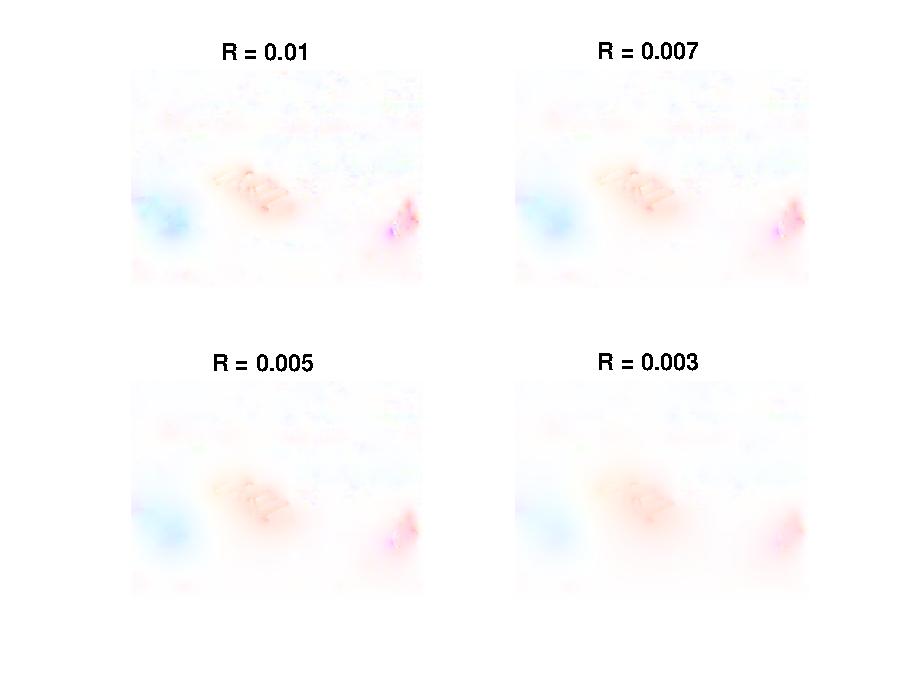
\includegraphics[scale=0.8]{regularizationHS}
%    \caption{Different choices for regularization parameter $\sigma$ using the Horn and Schunck algorithm}
%    \label{reguHS}
%\end{figure}
%
%\begin{figure}
%    \centering
%    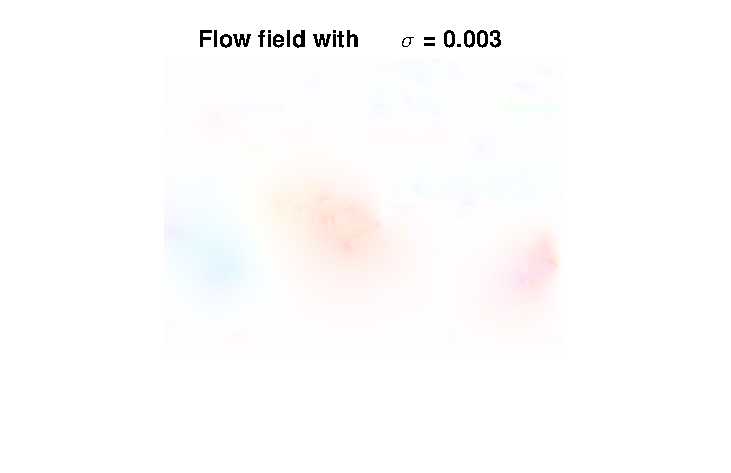
\includegraphics[scale=1]{HSregu}
%    \caption{Flow field with $\sigma= 0.003$ using the Horn and Schunck algorithm}
%    \label{reguHS_best}
%\end{figure}




\section{Anisotropic image-driven regularization}
\chapter{Anisotropic Image-Driven Regularization}
\sectionmark{Anisotropic Image Driven Regularization}
The homogeneous regularizer of Horn and Schunck smoothes the flow field in all directions. This is a desirable property for internal pixels of an object, but not for pixels on the flow boundary. A homogeneous regularizer would smooth the flow field at pixels where one would expect the flow field to be discontinuous, which results in blurry flow edges. 
\section{Regularization according to image structure}
As one of the assumptions to the optical flow model is that different object has different brightness patterns, one would expect that flow boundaries coincide with image edges. Thus an amendment to this issue is to make a smoothness term which takes the gradients of the image into account, and smooths the flow field along image edges instead of across them. Such methods are called image-driven regularization methods. The anisotropic reguralizer of Nagel and Enkelmann \cite{Nagel:1986:ISC:11284.11285} performs smoothing along the image gradients and prevents smoothing across image edges. This is done by introducing a regularised projection matrix $P$, defined as
\begin{align*}
P(\nabla f) = \frac{1}{|\nabla f|^2 + 2 \kappa^2} (\nabla^{\bot} f (\nabla^{\bot})^T + \kappa^2 I),
\end{align*}
where $\nabla^{\bot} f= \left[-f_y, f_x \right]^T$, and $\kappa > 0$ is a regularization parameter. The smoothness term of Nagel and Enkelmann can now be written as the following
\begin{align*}
V_{AI}(\nabla u, \nabla v) = \nabla ^T u P(\nabla f) \nabla u + \nabla ^T v P(\nabla f) \nabla v,
\end{align*}
or written out 
\begin{align*}
V_{AI}(\nabla u, \nabla v) = \frac{\kappa^2}{|\nabla f|^2 + 2 \kappa^2} \left( u_{\textbf{s}_1}^2 + v_{\textbf{s}_1}^2 \right) + \frac{|\nabla f|^2 + \kappa^2}{|\nabla f|^2 + 2 \kappa^2} \left(u_{\textbf{s}_2}^2 + v_{\textbf{s}_2}^2 \right),
\end{align*}
where 
\begin{align}
\label{ID_smoothingDir}
&\textbf{s}_1 = \frac{1}{|\nabla f|}\begin{bmatrix}
f_x \\
f_y
\end{bmatrix},
& & \textbf{s}_2 = \frac{1}{|\nabla f|}\begin{bmatrix}
-f_y \\
f_x
\end{bmatrix}, & 
\end{align}
and $q_{\textbf{s}_i} = \textbf{s}_i^T \nabla u$ for $q = u, v$. That is, $q_{\textbf{s}_i}$ is the directional derivative of $q$ in the direction of the image gradient ($i=1$) or the orthogonal direction ($i=2$). This means that setting $\Theta=P$ in (\ref{EL_regu}) steers the diffusion so that flow vectors are smoothed along image edges and not across them.

\subsection{Discretizing the Nagel and Enkelmann smoothness term}
Setting $\Theta=P$ in (\ref{EL_regu}) leads to the following Euler-Lagrange system:
\begin{align*}
\frac{\partial M}{\partial u} - \frac{1}{\sigma^2} \text{div}(P \nabla u) = 0 \\
\frac{\partial M}{\partial v} - \frac{1}{\sigma^2} \text{div}(P \nabla v)= 0.
\end{align*}
Using the same discretizations for the derivatives as in \ref{sec: disc} one gets
\begin{align*}
(D^T D + \frac{1}{\sigma^2} L^TPL) \textbf{w} = - D^T \textbf{c}
\end{align*}
for the internal pixels and with Neumann boundary conditions given in equations (\ref{neumann1}) to (\ref{neumann8}). (Maybe some more details on discretization?)

\subsection{Results for the anisotropic image-driven regularization}
Experiments were run to find the best regularization parameter in the Nagel and Enkelmann smoothness term. The regularization parameter $\sigma$ found for the Horn and Schunck method is used to regularize the whole smoothness term. The resulting flow field for different choices of the regularization parameter $\kappa$, while keeping $\sigma$ constant, is shown in Figure (\ref{reguNE}). It is seen that choosing $\kappa = 0.8$ gives a fairly good segmentation of the object. Since the values for the gradient from the sobel derivative are relatively high, it is expected to also having to choose a relatively large value for $\kappa$ for sufficient regularization. Figure (\ref{reguNEHS}) compares the anisotropic smoothness term of Nagel and Enkelmann with $\kappa = 0.8$ with the homogeneous smoothness term of Horn and Schunck, both with using regularization parameter $\sigma = 0.003$. 

%\begin{figure}
%    \centering
%    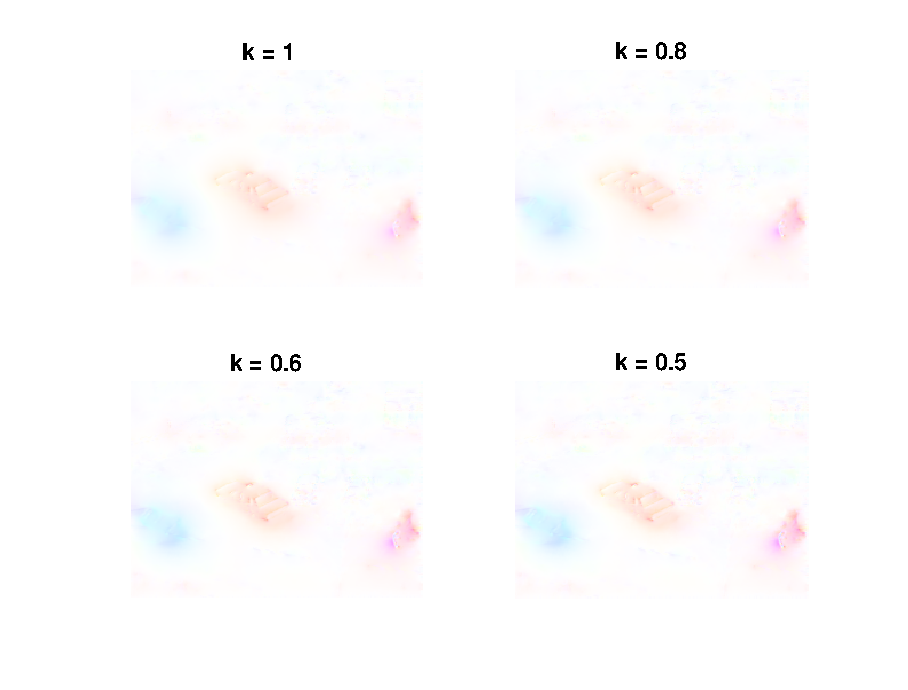
\includegraphics[scale=0.8]{regularizationNE.eps}
%    \caption{Different choices for $\kappa$ using the Nagel and Enkelmann smoothness term}
%    \label{reguNE}
%\end{figure}
%
%\begin{figure}
%    \centering
%    \includegraphics[scale=0.8]{NEregu}
%    \caption{Flow field with $\kappa= 0.8$ and $\sigma = 0.003$ using the Nagel and Enkelmann smoothness term.}
%    \label{reguNE_best}
%\end{figure}
%
%\begin{figure}
%    \centering
%    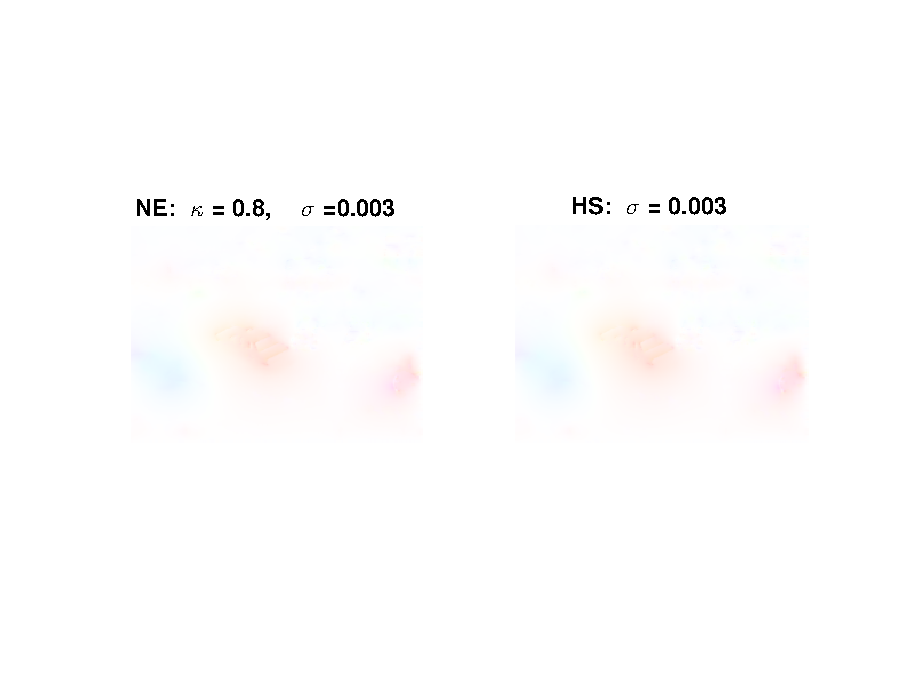
\includegraphics[scale=0.8]{reguNEHS.eps}
%    \subfloat[\label{NE_best} Anisotropic smoothness term.]{\hspace{.5\linewidth}}
%	\subfloat[\label{HS_best} Homogeneous smoothness term.]{\hspace{.5\linewidth}}
%	\caption{Comparison of the anisotropic and homogeneous smoothness term for given parameter choices.\label{humans}}
%    \label{reguNEHS}
%\end{figure}

\section{Isotropic Flow-driven regularization}
\chapter{The Isotropic Flow-Driven Method}
One drawback of the image-driven approach to regularization is that there is often a great deal of oversegmentation, since image boundaries are not necessarily flow boundaries. The solution is to decrease the smoothing on flow boundaries, a so called flow-driven approach. But an obvious problem is that the flow boundaries are not known a priori.
\section{Subquadratic Penalization}
Shulman and Herve \cite{ShulmanHerve} suggested using a subquadratic penalizer instead of a quadratic one, arguing that a quadratic penalizer assumes a Gaussian distribution of the flow gradients which would penalize large gradients, assumed to correspond to flow boundaries, too much. The smoothness term can be written as
\begin{align*}
V_{IF}(\nabla u, \nabla v) &= \psi_V \left( |\nabla u|^2 + |\nabla v|^2 \right) \\ 
&= \psi_V \left( u_{\textbf{s}_1}^2 + u_{\textbf{s}_2}^2 + v_{\textbf{s}_1}^2 + v_{\textbf{s}_2}^2 \right),
\end{align*} 
where $\psi_V(s^2)$ is some subquadratic penalizer function performing a nonlinear isotropic diffusion. The contribution to (\ref{EL}) is $\nabla \cdot (\partial_{u_x} V, \partial_{u_y} V)$. Computing the individual components, we get
\begin{align*}
\partial_{u_x} V = 2 \psi_V' \left( u_{\textbf{s}_1}^2 + u_{\textbf{s}_2}^2 + v_{\textbf{s}_1}^2 + v_{\textbf{s}_2}^2 \right) u_x \\
\partial_{u_y} V = 2 \psi_V' \left( u_{\textbf{s}_1}^2 + u_{\textbf{s}_2}^2 + v_{\textbf{s}_1}^2 + v_{\textbf{s}_2}^2 \right) u_y,
\end{align*}
and equivalent for $(\partial_{v_x} V, \partial_{v_y} V)$. Thus the diffusion matrix of (\ref{EL_regu}) is given as
\begin{align*}
\Theta_{IF} = 2 \psi_V'\left( u_{\textbf{s}_1}^2 + u_{\textbf{s}_2}^2 + v_{\textbf{s}_1}^2 + v_{\textbf{s}_2}^2 \right) I,
\end{align*}
where $I$ is the identity matrix, which is seen to be a function of the flow gradient. As a convex penaliser, Cohen (1993) suggested the following total variation regulariser:
\begin{align}
\label{TV_regu}
\psi_V(s^2) = \sqrt{s^2 + \epsilon^2},
\end{align} 
which gives
\begin{align*}
\psi_V'(s^2) = \frac{1}{2 \sqrt{s^2 + \epsilon^2}}.
\end{align*}
This penaliser function results in the following Euler-Lagrange system
\begin{equation}
\begin{aligned}
\label{EL_LD}
\partial_u M - \frac{1}{\sigma^2} \left(\frac{\partial}{\partial x}\left[ \frac{u_x}{\sqrt{|\nabla u|^2 + |\nabla v|^2  + \epsilon^2}} \right] + \frac{\partial}{\partial y} \left[ \frac{u_y}{\sqrt{|\nabla u|^2 + |\nabla v|^2  + \epsilon^2}} \right] \right) = 0 \\
\partial_v M - \frac{1}{\sigma^2} \left(\frac{\partial}{\partial x}\left[ \frac{v_x}{\sqrt{|\nabla u|^2 + |\nabla v|^2 + \epsilon^2}} \right] + \frac{\partial}{\partial y} \left[ \frac{v_y}{\sqrt{|\nabla u|^2 + |\nabla v|^2 + \epsilon^2}} \right] \right) = 0,
\end{aligned}
\end{equation}
which is clearly a non-linear system. (Something more about TV regularizers? Rudin et al.)


\subsection{The Lagged Diffusivity Fixed Point Method}
The non-linear system (\ref{EL_LD}) is can be solved using the method of lagged diffusivity. Chan and Mulet \cite{Chan1999} showed that the lagged diffusivity fixed point method used in TV restoration of images can be traced back to Weiszfeld's method of minimizing Euclidean lengths, and for which global and linear convergence can be shown. From (\ref{EL_LD}) we can define the fixed point method as
\begin{align*}
\partial_{u^{k+1}} M - \frac{1}{\sigma^2} \left(\frac{\partial}{\partial x}\left[ \frac{u^{k+1}_x}{\sqrt{|\nabla u^k|^2 + |\nabla v^k|^2 + \epsilon^2}} \right] + \frac{\partial}{\partial y} \left[ \frac{u^{k+1}_y}{\sqrt{|\nabla u^k|^2 + |\nabla v^k|^2 + \epsilon^2}} \right] \right) &= 0 \\
\partial_{v^{k+1}} M - \frac{1}{\sigma^2} \left(\frac{\partial}{\partial x}\left[ \frac{v^{k+1}_x}{\sqrt{|\nabla u^k|^2 + |\nabla v^k|^2 + \epsilon^2}} \right] + \frac{\partial}{\partial y} \left[ \frac{v^{k+1}_y}{\sqrt{|\nabla u^k|^2 + |\nabla v^k|^2 + \epsilon^2}} \right] \right) &= 0,
\end{align*}
where we solve for $u^{k+1}$ and $v^{k+1}$ given $u^k$ and $v^k$ from the previous iteration. This is a linear system in each iteration, and it can be solved in the same manner as the previous methods. The system to be solved at iteration $k+1$ is
\begin{align*}
(D^T D + \frac{1}{\sigma^2} L^T\Theta^{k}L) \textbf{w}(\xi)^{k+1} = - D^T \textbf{c}(\xi),
\end{align*}
for $\xi \in \Omega$, where $\Theta^k$ is the following 4mn-by-4mn diagonal block matrix
\begin{align*}
\Theta^k = \left[
\begin{array}{c|c|c|c}
\chi^k & 0 & 0 & 0 \\ \hline
0 & \chi^k & 0 & 0 \\ \hline
0 & 0 & \chi^k & 0 \\ \hline
0 & 0 & 0 & \chi^k
\end{array}
\right].
\end{align*}
The submatrix $\chi^k$ is the mn-by-mn diagonal matrix with the values 
\begin{align*}
\chi^k_i &= 2 \psi_V'\left( |\nabla \textbf{w}(\xi^i)|^2 \right) \\
& = \frac{1}{\sqrt{|\textbf{w}(\xi^i)|^2 + \epsilon^2}}
\end{align*}
along its diagonal.

\subsection{Results for Isotropic flow driven}
....


  

%\begin{thebibliography}{}
%
%\bibitem{Chan}
%Chan, T. and Mulet, P. (1999) On the convergence of the lagged diffusivity fixed point method in total variation image restoration. \emph{SIAM Journal of Numerical Analysis} (Vol. 36, No. 2, pp 354-367)
%
%\bibitem{Cohen}
%Cohen, I. (1993). Nonlinear variational method for optical flow computation. \emph{Proceedings. Eighth Scandinavian conference on Image Analysis} (Vol. 1, pp. 523–530). Norway, Tromsø.
%
%\bibitem{CH}
%Courant, R. and Hilbert, D. (1953). Methods of Mathematical Physics. Vol. I (First English ed.), Interscience Publishers, New York
%
%\bibitem{Courant}
%Courant, R. (1947). Differential and Integral Calculus, Vol. II, 2nd edition, Interscience Publishers, New York
%
%
%\bibitem{HS}
%Horn, B. and Schunck, B. (1981). Determining optical flow. \emph{Artificial Intelligence}, 17, 185-203.
%
%\bibitem{NE}
%Nagel, H. and Enkelmann, W. (1986). An investigation of smoothness constraints for the estimation of displacement vector fields from image sequences. \emph{IEEE Transactions on Pattern Analysis and Machine Intelligence}, 8, 565-593
%
%\bibitem{SH}
%Shulman, D. and Hervé, J. (1989). Regularization of discontinuous flow fields. \emph{Proceedings. Workshop on Visual Motion} (pp. 81–86). Irvine: IEEE Computer Society Press.
%
%\bibitem{OFH}
%Zimmer, H., Bruhn, A., Weickert, J. (2011). Optic Flow in Harmony \emph{International Journal of Computer Vision}, 93, 368-388
%
%
%\end{thebibliography}
%

\printbibliography

\end{document}

